\chapter{Methode en technieken}
Dit hoofdstuk zal verschillende methode, technieken en tools beschrijven die gebruikt zijn tijdens het project. Voor elke tool zal er beschreven woorden waarom voor een bepaalde methode, techniek en tool gekozen is. Er zal als eerst gekeken worden naar de methode, vervolgens de technieken en uiteindelijke de tools.

\section{Methode}
In het hoofdstuk wordt er gekeken naar alle methodes die gebruikt zijn tijdens het uitvoeren van het project. Daarnaast wordt er ook beschreven waarom ze gebruikt worden.

\subsection{HBO-I methodes}
Tijdens de afstudeerstage zal er gebruikt gemaakt worden van twee onderzoeksmethodieken, ten eerste zal er \textit{Hardware validation onderzoek} gebruikt worden voor de hardware validatie. De andere onderzoeksmethodiek is \textit{Design Pattern research}, dit zal gebruikt worden voor het generieke software ontwerp te ontwikkelen\parencite{researchmethods}. Hardware validation onderzoek is gekozen om een uiteindelijke testplan te ontwikkelen om het hardware te kunnen testen. Design Pattern research zal gebruikt worden om een duidelijk en generiek structuur van de applicatie te ontwikkelen. Hiervoor zal verschillende design patterns gebruikt worden. Voor de volgende deelvragen zal \textit{Design Pattern research} gebruikt worden: 
\begin{enumerate}
	\item De Satellite heeft een robuuste communicatie over CAN en UDP.
	\item Generiek en modulair opgebouwd software, waardoor het in de toekomst makkelijk uitgebreid kan worden.
\end{enumerate}

\noindent De laatste deelvraag zal beantwoord worden met \textit{Hardware validation onderzoek}:
\begin{enumerate}
	\item De Satellite IO porten zijn volledig getest, en kunnen communiceren met sensoren. Dit wordt gedaan aan de hand van een testplan.
\end{enumerate}

\subsection{Werkmethoden}
Om er voor te zorgen dat alle eisen en doelstelling gehaald worden is er van belang om te kiezen voor een goed werkmethode voor het project. Werkmethodes zorgen ervoor dat het project efficient en succesvol gedraaid worden. Er zijn verschillende werkmethodes bedacht, maar tijdens de stage is er een selectie gemaakt uit drie werkmethoden. De drie werkmethode zijn V-Model, waterval en Agile. Deze drie zijn gekozen omdat de stagair hier al ervaring mee heeft. Dit betekent dat er geen nieuwe methodes geleerd hoeven te worden. \newline

\noindent Uiteindelijk is er gekozen voor een combinatie tussen Waterval en Agile. Dit is omdat er vaste eisen en taken zijn gespecificeerd door de klant, die heel makkelijk opgesplitst kunnen worden in kleinere taken. Van de waterval methode worden fases meegenomen die gaan als volgt. Als eerst komt de requirements, design, implementatie, verificatie en maintenance. De maintenance fases zal buiten de scope van het stage vallen. Er is gekozen voor Agile aangezien het niet duidelijk vanaf het begin welke taak als eerst geïmplementeerd moet worden. Dit zal dan besproken worden elke twee weken, en meerdere keren per week zal er besproken worden hoe het voortgang is. Hieronder is een overzicht \ref{fig:agilewaterval} dat een beeld geeft hoe de fases zullen lopen.

\begin{figure}[h!]
	\centering
	\caption{Werkmethode}
	\label{fig:agilewaterval}
	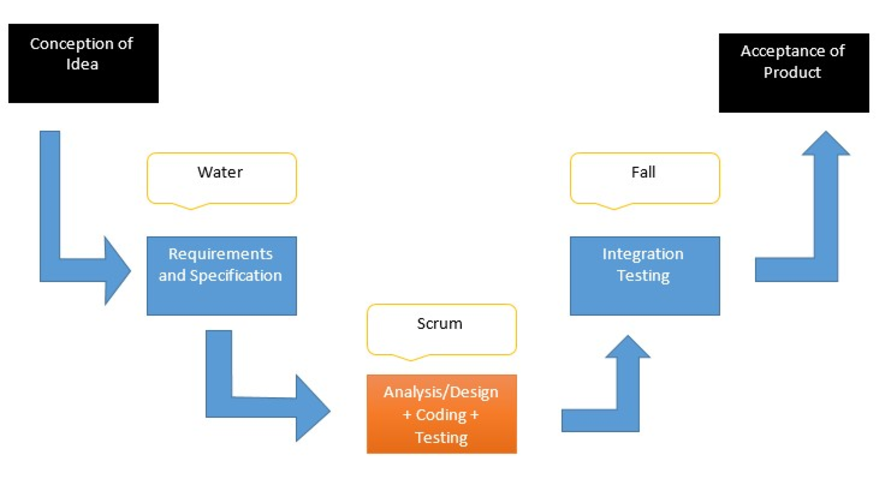
\includegraphics[width=0.7\linewidth]{methodetechnieken/werkmethoden/water-scrum-fall-diagram.png}
\end{figure}


\section{Technieken}
Er is als eerst gekeken naar een van de belangrijkste techniek van softwareontwikkeling, de programmeertaal. Elke taal heeft zijn voordelen en nadelen, er moet dus ook goed bekeken worden of een taal wel gebruikt kan worden voor embedded softwareontwikkeling. In Sensor Maritime worden een aantal talen standaard gebruikt, dat is C en C\#. Omdat het product in de toekomst nog aangepast kan worden is er niet gekeken naar andere talen zoals bijvoorbeeld Rust. Hiervoor is gekozen omdat de toekomstige developer deze taal dan zou moeten kennen. De hardware abstractielaag van de microcontroller is standaard geschreven in C. Daarnaast levert de Infineon IDE standaard een C compiler. Met C zal dan uiteindelijke ook implementatie gedaan worden. Er is niet gekeken voor externe compilers voor C\# voor ARM based systemen aangezien je dan niet weet wat de ondersteuning en robuustheid ervan is. Daarnaast was ook gekeken naar de C++, aangezien het embedded systeem het standaard ondersteund, maar omdat binnen Sensor Maritime meer ervaring is met C, is er voor C gekozen. 

\section{Tools}
Tijdens de afstudeerstage zijn er een aantal verschillende tools gebruikt voor de implementatie en ontwerp van het project. De tools opgesplitst in het ontwerp en implementatie van het software.

\subsection{Ontwerp}
\begin{enumerate}
	\item Astah \\ Hiermee is verschillende UML diagrammen ontwikkeld, zoals de klassediagram en statemachines.
\end{enumerate}
\subsection{Implementatie}
\begin{enumerate}
	\item DAVE \\ DAVE is de standaard gemaakte IDE van Infineon, het heeft dus ook APP support waardoor je de hardware makkelijk kan configureren.
	\item GitHub (Git) \\ De standaard versiebeheer wat Sensor Maritime gebruikt.
	\item Segger J-Link \\ Met de J-Link kon er gebruikt gemaakt worden van debuggen, dit betekent dat dat je makkelijk weet waar de programma mee bezig is.
	\item Trello \\ De agile bord waarop alle sprints en taken bijgehouden wordt.
\end{enumerate}

